In this chapter we will present two applications that have been implemented with our Precision Timed Architecture.
The first application is a real-time one dimensional computational fluid dynamics (1D-CFD) simulator.
This simulator runs in real-time to simulate the fuel rail pressure and flow rate for improved engine efficiently when injecting fuel.
The application makes use of the light weight hardware threads in our thread-interleaved pipeline to implement a massively parallel simulator with hundreds of computational nodes communication to its neighbors.
The timing predictable architecture allows us to statically analyze the execution time for each node to ensure that the execution time for each computational node can meet the timing constraints imposed by the application.
A timed base communication scheme is implemented to reduce communication overhead.
The communication synchronization is enforced in software with timing instructions to minimize overhead and enforce that communication occurs on-time and all nodes are in sync.  
We present the synthesis results on a Xilinx Virtex-6 FPGA to show that we can simulate an engine fuel rail configuration of up to 400 nodes.       

The second application shows how we use our predictable architecture to eliminate timing side-channel attacks for encryption algorithms.
Time-exploiting attacks take advantage of variations in execution time of cryptosystems to deduce the encryption keys.
The root cause of these time-exploiting attacks is the uncontrollable run-time variance that is caused by the underlying architecture, allowing attackers to bypass the strong mathematical properties of the encryption and deduce the keys.   
We show that by using a timing-predictable architecture that provides more control of execution time to the programmer, we remove the vulnerability that is used to initiate the attack, and remove architecture deficiencies that can lead to more timing-attacks.    
We demonstrate this by running RSA and DSA encryption algorithms on PRET, which successfully illustrates the use of PRET�s timing-centric methods to counter time-exploiting attacks.
 
\section{Real-Time 1D Computational Fluid Dynamics Simulator}
\label{sec:1dCFD}

Modern diesel engines inject diesel fuel with high pressure into the combustion chamber for combustion.
A digital control value is used to control the amount of fuel injected, which depends on the pressure and fuel rate of the fuel rails delivering the fuel.   
Several pilot injections are injected ahead of the main injection to mitigate the inject delay in the chamber and reduce audible noise.
However, these pilot injections send pulsations through the fuel supply rail that need to be modeled or damped before subsequent injection events to ensure the correct amount of fuel is injected~\cite{BoschDiesel}. 
Currently, fuel rails are modeled and developed with 1D-CFD solvers like GT-Fuel, and use an ad-hoc model of fuel pressure for injection events~\cite{Winward01082010}.
1D-CFD models are commonly used in simulating transient operation of internal combustion engines \cite{SAE2009010695}.  
Here, we present an implementation for real-time execution of a 1D-CFD solver using multiple PRET cores that model the fuel rail.
Although the calculations are slightly rougher than the GT-Fuel calculations, it is sufficient to allow improved fuel pressure estimation and close the loop of fuel delivery, allowing for a cleaner, more efficient engine.     


\subsection{Background}
The 1D CFD model of the fuel rail system is descried as a network of pipes.
The system is built up from different types of pipe segments, which each model the fluid dynamics of a segment in the fuel rail.   
A fixed time step solver is implemented.
At each time step, the pipe segments calculate its current pressure and flow-rate, and communicate these to its neighboring pipe segments to be used in the next time step. 
The time step is determined by the speed of information flow that is expressed in equation \ref{Courant}.
\begin{equation} \label{Courant}
\frac{\Delta t}{\Delta x}a = C
\end{equation}
In this equation, \(a\) is the wave speed, \(C\) is the Courant number and \(\Delta x\) is the descretization length.  
For stability, the Courant number needs to be less than 1 and a number below 0.8 is recommended~\cite{GTFuel}.
For example, if a fluid has a wave speed \(a\) of 1 $cm$ per microsecond and a discretization length \(\Delta x\) of 1 $cm$, then we require a time step \(\Delta t\) of less than one microsecond.  
This discretization length of a pipe network is dominated by its smallest sub-volume and a 1 $cm$ discretization length is common for diesel fuel systems.  
For diesel engines, a speed of sound (wave speed) of 1500 $m/s$~\cite{DieselSpeedOfSound} is commonly used.
The real-time requirements of this application thus require adequate performance so that the slowest node can complete in \(\Delta t\).
Although highly parallel, the heterogeneity of pipe elements differentiates this application from typical homogeneous parallel problems often solved using GPUs or SIMD with large common memories~\cite{10.1109/FCCM.2006.20}, such as in image processing applications.

\begin{table}[b]
\begin{center}
\begin{smalltabular}{|l|c|c|}
\hline
\textbf{Type} 							& \textbf{(\emph{Pressure}) $P_{I_n}=$}										& \textbf{(\emph{Flow Rate}) $Q_{I_n}=$} \\ 
\hline
Pipe Segment  						&$\frac{\left(C_P+C_M\right)}{2}$ 				&$ \frac{\left(P_{I_n}+C_m\right)}{B}$ \\ 
\hline
Imposed pressure 							&$\scriptstyle P_{Bnd}$ 							&$\frac{(P_{Bnd}-C_M)}{B}$ \\
\hline
Imposed mass flow  							&$\scriptstyle C_M+BQ_{Bnd}$ 					&$ \scriptstyle Q_{Bnd}$ \\
\hline
\multirow{3}{*}{Valve} 		&\multirow{3}{*}{$\scriptstyle C_P-BQ_{I_n}$}	&$\scriptstyle -BC_V+\sqrt{(BC_V)^2+2C_VC_P}$ \\ 
 								&													&$\scriptstyle C_V=\frac{(Q_0 \tau)^2}{2P_0}$\\ 
\hline
Cap 							&$\scriptstyle C_P-BQ_{I_n}$ 					&$\scriptstyle 0$ \\ 
\hline
\multirow{3}{*}{``T" intersection} 	&\multirow{3}{*}{$\frac{\frac{C_{P_1}}{B_1}+\frac{C_{M_2}}{B_2}+\frac{C_{M_3}}{B_3}}{\sum \frac{1}{B}}$} &$-\frac{P_I}{B_1}+\frac{C_{P_1}}{B_1}$ \\ 
 								&  													&$-\frac{P_I}{B_2}+\frac{C_{M_2}}{B_2}$\\ 
 								& 													&$-\frac{P_I}{B_3}+\frac{C_{M_3}}{B_3}$\\ 
\hline
\end{smalltabular}
\caption{Table of supported pipe elements and their derived equations} 
\label{tab:1dcfd_pipe_types}
\vspace{-8mm}
\end{center}
\end{table}

In order to evaluate our system of pipes we define a few types of computing nodes that corresponding to different pipe elements.
These are shown in table~\ref{tab:1dcfd_pipe_types} with derived pressure and flow rate equations.
From these pipe elements we can generate a network of pipes that represent our fuel system.  
The \emph{imposed pressure} is used to represent the pressure sensor on the fuel system. 
The \emph{imposed mass flow} is used to represent pump, and the \emph{valve} is typically used to represent an injector.
\emph{Pipe segments} and \emph{pipe ``T''} are the interconnected pipe elements, and the \emph{cap} is used to represent the end of a pipe.
The derived equations shown in the table use the following simplified characteristic equations derived in~\cite{viele20121dcfd}.  
\begin{equation}
C_P=P_{i-1}+Q_{i-1}\left(B-R|Q_{i-1}|\right) \text{ and}
\end{equation}
\begin{equation}
C_M=P_{i+1}-Q_{i+1}\left(B-R|Q_{i+1}|\right).
\end{equation}
In the equations, \(B = a\rho / A\) and \( R=\rho f \Delta x/2DA^2\), where \(A\) is the cross sectional area of the pipe, and \(Q\) is the flow rate along the pipe.
\(P\) is pressure, \(\rho\) is fluid density, \(V\) fluid velocity, \(f\) is the Darcy-Weisbach friction factor, \(D\) is pipe diameter, and \(a\) is the wave speed.
The $_{Bnd}$ subscript denotes a boundary condition.  
$C_v$ is the flow coefficient which is a function of: $Q_0$ the nominal open flow, $P_0$ the downstream pressure, and $\tau$ the fraction the valve is open. 
The $_{i+1}$ subscript and $_{i-1}$ subscript represent values that are received from the neighboring pipe elements.
Any implementation of the system must ensure that these calculations for all pipe elements can be completed within the specified time step.
  
\begin{figure}
\noindent\makebox[\textwidth]{
\begin{minipage}[b]{0.55\linewidth}
\centering
\includegraphics[page=22,scale=0.6]{./figs/1dcfd/FCCM2012Figures.pdf}
\caption{Design Flow}
\label{fig:1dcfd_design_flow}
\end{minipage}
\hspace{0.5cm}
\begin{minipage}[b]{0.45\linewidth}
\centering
\includegraphics[page=7, scale=0.5]{./figs/1dcfd/FCCM2012Figures.pdf}
\caption{High Level System Diagram}
\label{fig:1dcfd_HighLevelDiagram}
\end{minipage}
}
\end{figure}

Figure \ref{fig:1dcfd_HighLevelDiagram} shows an overview of a representative system for modeling fuel rails.  
The 1D CFD model is bounded inside the dashed rectangle.  
External to that is the real-word sensor and actuator interfaces that provide boundary conditions or consume model output variables.  
The small blue squares inside the dashed rectangle represent the network of pipes.  
In a practical simulation of a diesel fuel system the total number of pipe elements can range from around 50 to a few hundred.  
The configuration of the network of pipes depends on the actual fuel rail being modeled.

The design flow of the system is shown in figure~\ref{fig:1dcfd_design_flow}.
Starting from a description of the flow system and our library of elements we  create a graph to describe the system.  
The flow system will also dictate the maximum time step of the system.  
With this information we can instantiate processors and interconnects tailored to our needs and apply the library code to them.
From there we can build and deploy our system.


\subsection{Implementation}
Each pipe element is a computational node, and their graphical representation is shown in Table~\ref{CELibrary}. 
The top 3 rows of the table represent the flow elements described in Table~\ref{types}.  
%The 4th row contains two helper functions that also run on threads of processors.  
{\em Mechanical calculation} elements compute the inputs to valve, defined flow, and defined pressure blocks.
They serve as an interface between the flow model and the real world.
{\em Global calculation} elements are used to compute the temperature dependent variables of density and wave speed. 
They post their data to a global distribution node, broadcasting it to all other nodes.
Blocks with white backgrounds in the last row of Table~\ref{CELibrary}, i.e., {\em Global distribution} and {\em Output} denote that they are implemented directly in FPGA fabric, not mapped to a processor thread.  
Global distribution elements are purely used to indicate a distribution of input value to each of the computational elements in our model.
Output elements are used when data needs to be communicated out of the model to other parts of the FPGA. 

For illustrative purposes, we show a simplified sample pipe network with an imposed flow input (P1) in Fig.~\ref{DetailedDiagram}. 
Fluid travels through a few pipe segment nodes (P2 and P3) to a ``T" intersection (P4), where it splits off to a second branch of the network.
The ``T" node is also measured by the outside world (D1) through a output port.  
Flow going up the new leg ends in a cap (P8), while flow continuing down the original path exits the system through a valve (P6).  
The system is assumed to be at uniform temperature and values based on the temperature dependent variables of density and wave speed are computed by global calculations (G1, G2, and G3) and delivered by global distributions (GD1, GD2, and GD3) to each of the computational elements every time step for use in the subsequent time step.
%For the purposes of system analysis we assume that flow always enters through the left and exits to the right and possibly top of the network element.  This lets us describe the system as a directed graph of the form in Section \ref{sec:mapping}. 
%Since global values are delivered to every node they may be omitted from our graph representation.
%
%
\begin{table}
\begin{center}
\caption{Library of Computational Node Elements}
\begin{tabular}{|p{2.7cm}|c|p{2.7cm}|c|}
\hline
Pipe segment				&\includegraphics[page=11, scale=0.25]{./figs/1dcfd/FCCM2012Figures.pdf} &
Cap 						&\includegraphics[page=12, scale=0.25]{./figs/1dcfd/FCCM2012Figures.pdf} \\ \hline
Imposed pressure 			&\includegraphics[page=13, scale=0.25]{./figs/1dcfd/FCCM2012Figures.pdf} &
Imposed flow 				&\includegraphics[page=14, scale=0.25]{./figs/1dcfd/FCCM2012Figures.pdf} \\ \hline
Pipe ``T" 					&\includegraphics[page=15, scale=0.25]{./figs/1dcfd/FCCM2012Figures.pdf} &
Valve 						&\includegraphics[page=16, scale=0.25]{./figs/1dcfd/FCCM2012Figures.pdf} \\ \hline
Mechanical calculation	&\includegraphics[page=17, scale=0.25]{./figs/1dcfd/FCCM2012Figures.pdf} &
Global calculation 		&\includegraphics[page=18, scale=0.25]{./figs/1dcfd/FCCM2012Figures.pdf} \\ \hline
Global distribution 		&\includegraphics[page=19, scale=0.25]{./figs/1dcfd/FCCM2012Figures.pdf} &
Output 					&\includegraphics[page=20, scale=0.25]{./figs/1dcfd/FCCM2012Figures.pdf} \\ \hline
\end{tabular}
\label{CELibrary}
\end{center}
\end{table}


%
\begin{figure}
\centering
\includegraphics[page=3, width=0.49\textwidth]{./figs/1dcfd/FCCM2012Figures.pdf}
\caption{Detailed System Diagram}
\label{DetailedDiagram}
\end{figure}
%

\subsection{System Hardware Architecture} 
\label{sec:hardware_architecture}
The hardware architecture of real-time 1D CFD evaluation consists of multiple PRET cores connected through point-to-point connections and a global distribution circuit.
Fig.~\ref{ARM_Cores} shows a block-level view of the hardware architecture.   
As mentioned in Section \ref{sec:PRET}, each core consists of hardware threads interleaved through the pipeline in a predictable round robin fashion.
Computational nodes are mapped onto hardware threads, instead of each being implemented as its own core.
%This saves on the resources required for each node to implement its own dedicated datapath.  
This provides two major advantages.  
First, multi-threaded architectures maximize the throughput over latency.  
Multi-threaded architectures hide the latencies of multi-cycle operations, such as floating point operations or memory operations. 
When a hardware thread is waiting on these operations to complete, other threads can continue to execute in the pipeline.
E.g., in our implementation, floating-point addition and subtraction appear as single cycle instructions in timing analysis because the floating-point latency is hidden through the execution of other thread contexts within the pipeline. 
%The thread-interleaving further maximizes throughput by enforcing a round robin schedule of thread execution.  
%In our implementation, all floating point operations except square root and divide appear as single-cycle instructions during timing analysis.      
%of floating point units to make normally  appear as single-cycle instructions when timing analysis is done on individual threads. 
%Normally multi cycle instructions could now appear to be single-cycle when doing timing analysis on individual threads. 

%pipelined instructions like divide can appear as single step instructions to their respective thread.  
Second, the thread interleaved pipeline design allows for a simpler pipeline design.
Since data and control hazards are no longer present in the pipeline, the logic used for handling them can be stripped out, greatly reducing the cost of the core.
Furthermore, multiple threads share the same datapath, so the cost of adding threads is far less than adding a core, further reducing the cost of the system.
We discuss in more details the trade-offs involving adding threads later in Section~\ref{sec:results}.
%IL{Talk about how different hardware resources can be synthesized}
The memory footprint required for each node is small enough, roughly a hundred assembly instructions, so that the scratchpad is sufficient for memory use and no main memory is needed.

Only basic single-precision floating point operations (add/sub/multiply) are needed for most nodes. But some require more complicated operations:  
the valve element uses floating point square root and the ``T" element uses floating point divide, as shown in Table \ref{types}.
However, these elements typically represent only a few percent of the overall system.  
In our complex example presented later, the common rail fuel system, there are 234 nodes: only 5 nodes are ``T"s (requiring division) and 4 node are valves (requiring square root), which is approximately $4\%$.
To save on hardware resources, we could use software emulation for the complex operations. 
%This way we don't need to synthesize extra hardware for each core, which would only be used by the small percent of nodes that need it.  
However, our system is bounded by the slowest computational element, so the performance hit from using software emulation for these small percent of nodes would limit the overall real-time performance. 
But if we add hardware units on all the cores, it would be wasted on most cores with a homogeneous multi-core approach.
%In a homogeneous core approach, we would need to add hardware units to all cores if we required the performance for the few nodes. 
Instead, we adopt a heterogeneous multi-core approach and provide several configurations of the core that includes different floating point hardware units.
%The mapping algorithm described in Section~\ref{sec:mapping} uses this to optimize the resources used in the system by grouping nodes with similar functionalities onto the same core. 
We only synthesize hardware accelerators to the cores that require them. 
Since the number of cores which need hardware accelerators is small, we still get the throughput improvement from adding hardware support without the huge resource overhead. 
This justifies substantial resource savings, which we show in Section~\ref{sec:results}.  

%our approach adds hardware support for square root and divide only to the cores that contain a valve or ``T'' element.
%We describe in more detail the optimization and mapping algorithm in section~\ref{sec:mapping}. 
\begin{figure}
\centering
\includegraphics[page=8, width=0.49\textwidth]{./figs/1dcfd/FCCM2012Figures.pdf}
%\caption{System of Multi-threaded PRET Cores and Interconnects}
\caption{System of PRET Cores and Interconnects}
\label{ARM_Cores}
\end{figure}

%The heterogeneity of the nodes allows us to configure the cores according which nodes are mapped onto the cores. 
%\IL{Talk about different features for the core - floating point, fixed point, square root, divide} 
%We show in section~\ref{sec:results} the resources used for the different configurations of our core.
 
Each node in our system requires one to four input ports along with one to four output ports depending on the number of neighboring connections connected to its neighboring nodes.  
%The input ports are labeled "Left", "Right", "Top", and "Global" by default though they are overloaded as necessary for specific functions, for instance the valve node uses the top port to input valve position.
One input port is dedicated as the global port, which always receives broadcasts from the global distribution circuits.
Since only local communications occur across nodes, only point-to-point communication channels need to be established. 
%A complicated interconnect between all cores is not needed. 
%We only need to establish point-to-point communication channels between a core and its neighbors to ensure communication for the nodes mapped on the threads.
Nodes mapped to the same core (intra-core communication) can communicate through the shared local memory within the core as shown in Fig.~\ref{ARM_Cores}.
Nodes mapped to different cores (inter-core communication) communicate through the point-to-point interconnect as illustrated in Fig.~\ref{ARM_Cores}.  
We use shared dual-port Block RAMs (BRAMs) for our inter-core communication.
This serves two purposes. 
First, it provides single-cycle deterministic communication, as BRAM access is single cycle.
This allows the timing analysis to be simplified, as there is no hardware protocol that needs to be accounted for when accessing data through the inter-core communication channels. 
More importantly, the timing analysis for each node is now independent of the node mapping; both intra- and inter-core communication mechanisms are single-cycle, as they both access BRAMs.
If this were not the case, then the timing analysis needs to assume all communications are inter-core communications, i.e., the longer of the two. 
Second, by using the dedicated BRAM blocks on the FPGA for interconnects, we save the logic slices to be used for computation nodes.
This is useful because the limiting resource in our implementation is logic slices, not BRAMs, as justified later in Section~\ref{sec:results}.
%BRAM blocks are specialized resource blocks on the FPGA that are used to synthesize fast memory.
Each core only requires a small number of BRAMs to be used for registers and scratchpads, so the BRAM utilization ratio is far less than the logic slice utilization ratio.
At each time step only two words, pressure and flow rate values, are transferred from a node to each of its neighbors. 
Our time periodic execution of computation nodes(described next in Section~\ref{sec:software_architecture}) ensures that we only need a buffer size of one for each of the words. 
Because the communication bandwidth is small, we only need one BRAM block to establish an interconnect that allows all threads from one core to communicate with all threads on the other.

%By using precision timing to achieve data synchronization, this allows us to use simple hardware mechanisms such as a single BRAM to establish a single buffer for communication while ensuring no data races between nodes.   
%\IL{Make sure to explain why you don't need handshaking protocols in hardware, because we're doing it in software}  

%In our diesel fuel system implementation we assume all nodes are at the same temperature and compute the temperature dependent parameters wave speed and density globally.  
%Our system derives 3 temperature dependent parameters in an optimized form, and broadcasts them to every pipe element.   
All of our flow elements have a dependency on density and wave speed that are functions of temperature.  
Temperature is assumed to be the same throughout the system, so these parameters are computed in a single computational element and broadcast to all pipe elements through the global distribution circuit as illustrated in Fig.~\ref{DetailedDiagram}.
%For the global distribution circuit, we observe that most nodes only need to receive the broadcast; only a few nodes are sending the broadcast.  
%In fact, in diesel fuel systems, the number of parameters that need to be broadcast can always be fitted into a single core \IL{Matt, is this valid assumption? Is there a better way to state this?}.
%These 3 parameters are delivered to every pipe element.
Leveraging this, the global distribution circuit is implemented by a single broadcaster that writes to dedicated memories local to each core.
This broadcast receiving memory is synthesized to a small dual-port BRAM, with a read-only side connected to the core, and a write-only side connected to the broadcaster.
This memory is shared amongst all threads in a core so all threads can access the global values.
% of an extra dual ported BRAM at each core.
%All  and a single broadcast bus with that allows a dedicated core to write to the small local buffers.
%the broadcast receiving memories can all receive the broadcast and write in the broadcast values within a single cycle.
%The buffer can only be written from the broadcast bus and is read-only from the cores.
%The small local buffers are memory mapped on each core and can be accessed by all threads on the core.
%The mapping algorithm described in section \ref{sec:mapping} ensures that nodes which require global broadcasting of data will be mapped to a thread on the dedicated broadcast core.
This architecture allows us to save on the resources needed to implement a full fledged interconnect routing system or any network protocol to be used for broadcasting. 

%On the left you can see a six-thread implementation of the basic PRET architecture where each thread has its own register set and shares the pipelined ALU and more memory in a time-sliced fashion.  
%Additional cores are shown in smaller scale on the right.  
%Data connections between cores are shown with solid arrows.
  
%In this simple diagram data connection is shown only from one core to the next in a clockwise fashion around the diagram.  
%In more complex situations each core can be connected to between one and all other cores in the system, but as the amount of interconnection increases the advantages of this model over a global memory model decrease. \IL{This is not true actually, managing a global memory when core numbers go up is very costly.}

%In order to optimize FPGA resources we look at the relative costs in FPGA gates of various components in the system.  
%First is the cost of additional threads per processor core. 
%In our implementation we used a 150MHz system clock speed with 6 threads, so this is our baseline for area in Table \ref{Cores_vs_features}.  
%This is then divided by the number of threads to get the virtual execution rate of the cores.  


% %
% Each of these computational elements represented in the library is instantiated on one thread of one of the processor nodes.  
%------------------------------------------------------------------------ 
\subsection{Software Design}
%\GW{This section explains the software design, that's why it's titled that\ldots, i don't think ``acheving precise timing'' is general enough, as achieving precise timing is merely a requirement}
%\subsection{\GW{Software Architecture}}
\label{sec:software_architecture}
%\GW{let's all give this section a bit more attention to make it easy to read. RTAS review complains about this. Possible with a different title.}
We implement the equations in Table~\ref{types} in the language C and compile it with the GNU ARM cross compiler~\cite{gnu-arm} to run on our cores. 
% In order to minimize the computation required, the equations are statically optimized.  
% The system is also assumed to be at a constant temperature measured by an external sensor.  
% The temperature dependent terms of wave speed and density are computed globally and passed to each of the nodes each time step. 
Columns 2-6 in Table \ref{InstructionCount} show the number of Multiply, Add/Subtract, Absolute Value, Square Root, and Divide operations required by each computational element after optimization.
Each computational node is executed on a hardware thread and data is exchanged only at the boundaries of the time steps to avoid data races. 
Fig.~\ref{fig:software_model} shows an example timeline view of the operations for each node.    
The execution for computational nodes (top in Fig.~\ref{fig:software_model}) during each time step consists of three phases:
%\begin{enumerate}
%  \item 
(1) Read in the pressure and flow rate values from neighbors as well as global values;
%  \item 
(2) Compute the output values;
%  \item 
(3) Send output values to neighbors to be used for next time step.
%\end{enumerate}
The global and mechanical calculation nodes do not need to read data from other nodes, but might gather data from physical sensors and broadcast or send data to other nodes.  

\begin{figure}
\centering
\includegraphics[width=0.45\textwidth,page=5]{./figs/1dcfd/FCCM2012Figures.pdf}
\caption{Execution of Nodes at Each Time Step}
\label{fig:software_model}
\end{figure}
%\IL{There are several software implementations for a periodic execution model, but the execution time analysis of each node is crucial to ensure that we can meet the imposed timing constraints. }
%Although , any complex software control structure would still require path exploration or loop bound analysis for accurate time analysis.
The computation done by each node consists of only a single path of execution, voiding the need for complex software analysis.
We leverage the PRET %architecture's 
precise architectural timing analysis, which provides exact execution time for the computation in the nodes. 
%If mutex or locks were used to synchronize communication, the complexity of timing analysis would greatly increase because the execution time would be heavily influenced by the actions of other threads. 
Data synchronization is handled by the synchronized periodic communication points, which enforces an ordering between the writing and reading of shared data.
This voids the need of any explicit synchronization methods, removing any overhead and unpredictability for communication.
%So reading and writing across nodes in our implementation are simply reads and writes to memory mapped locations. 
%Broadcasting data to all nodes is also implemented by writing to a specific memory address region. 
%As described in the previous section,   
These properties allow us to statically obtain an exact execution time for each computation node, which we show in the last two columns of Table~\ref{InstructionCount}. 
A {\em Thread cycle} is defined as a thread's perceived clock cycle.
To get the physical execution time, multiply the thread cycles by the number of hardware threads in the pipeline to get processor clock cycles, then convert the clock cycles to physical time according to the processor clock speed.  

In addition to statically assuring that the worst-case execution time meets the timing constraints specified, we also need to enforce that node executions remain synchronized.
Our approach uses specialized timing instructions provided by the PRET architecture to enforce the synchronized communication points for all nodes.
%The timing instruction will synchronize the phases of different computational nodes, ensuring communication occurs only at specified time points.   
%The overhead of these instructions is very low, as they are designed directly into the core~\cite{pret_cases08}.
Fig.~\ref{fig:software_model} shows the program synchronization points that our timing instruction enforces.
The hatched area in the figure denotes slack time that is generated by the timing instructions.
When a timing instruction is decoded, it first enforces the previously specified timing constraint, then it specifies a new timing constraint for the next code block. 
In the code, one timing instruction is used during initialization to specify the first timing constraint.
Then, timing instructions are inserted at the end of each code block.
When the code block completes and the timing instruction is reached, the processor enforces the previously specified time bound by stalling if needed.
Once the specified execution time is reached, the code will continue execution and the next timing specification is set.    
Each timing instruction takes 2 cycles because it manipulates a 64-bit value representing time. 
For our computational elements, 3 timing instructions are used each computation iteration, thus 6 cycles of overhead are introduced per time step.
The overhead is already included in our execution time analysis presented in Table~\ref{InstructionCount}.
The same effect can possibly be achieved with no overhead using instruction counting and NOP insertions.
This can certainly be done on any deterministic architecture such as PRET. 
However, NOP insertion is both brittle and tedious. 
Any change in the code would change the timing of the software and insertions need to be adjusted to ensure the correct number of NOPs is added.
Designs now are mostly written in programming languages like the language C and compiled into assembly, making it extremely difficult to gauge the number of NOPs needed at design time.
The timing instructions allow for a much more scalable and flexible approach. 
In a system with heterogeneous nodes and different execution times, the timing instructions allow us to set the same timing constraints in all nodes regardless of its contents.   

%Each timing instruction takes 2 thread cycles, and allows timing control at granularity of thread cycles.     
%Its precision however is at the order of tens of nanoseconds, providing a high precision at extremely low cost. 
%\IL{Rework a little the part on timing instructions}

\begin{table}
\caption{Computational Intensity of Supported Types}
\begin{center}
\begin{tabular}{|@{\hspace{1.5mm}}c@{\hspace{1.5mm}}|@{\hspace{1.5mm}}c@{\hspace{1.5mm}}|@{\hspace{1.5mm}}c@{\hspace{1.5mm}}|@{\hspace{1.5mm}}c@{\hspace{1.5mm}}|@{\hspace{1.5mm}}c@{\hspace{1.5mm}}|@{\hspace{1.5mm}}c|@{\hspace{1.5mm}}c@{\hspace{1.5mm}}|}
\hline
 & \multicolumn{6}{@{\hspace{1.5mm}}c@{\hspace{1.5mm}}|}{Without Interpolation / With Interpolation} \\
\hline
\multirow{2}{*}{Type}	&\multirow{2}{*}{Mul}	&\multirow{2}{*}{Add/}	&\multirow{2}{*}{Abs}	&\multirow{2}{*}{Sqrt}	&\multirow{2}{*}{Div}	&\multirow{2}{*}{Thread} \\ 
 			& 		&Sub 	& 		&		&		&cycles\\ 
\hline \hline
Pipe segment					&10 / 18	&5 / 13		&2 / 2		&0 / 0 		&0 / 0		&81 / 51 \\ 
\hline
Imposed pressure 						&6 / 10		&3 / 7		&1 / 1		&0 / 0 		&0 / 0		&50 / 38 \\ 
\hline
Imposed flow			&5 / 9		&3 / 7		&1 / 1		&0 / 0 		&0 / 0		&51 / 40 \\ 
\hline
Valve 						&13 / 17	&5 / 9 		&1 / 1		&1 / 1 		&0 / 0		&64 / 55 \\ 
\hline
Cap 							&4 / 8		&2 / 6 		&1 / 1		&0 / 0 		&0 / 0		&48 / 39 \\ 
\hline
Pipe ``T" 		&16 / 28 	&13 / 25 		&3 / 0		&0 / 0 		&4 / 4		&111 / 72 \\ 
\hline  
\end{tabular}
\end{center}
\label{InstructionCount}
\end{table}


%%------------------------------------------------------------------------ 
%\subsection{Mapping Optimization}
%\label{sec:mapping}
%
%	Appropriately mapping a given problem to hardware resources is an important step to ensure that the FPGA device is used efficiently. Here we present a preliminary mapping algorithm that optimizes resource usage.
	  
%------------------------------------------------------------------------
%\subsubsection{Mapping Computational Graph to Processing Elements}
%The 1D CFD real-time simulation can be described as a directed graph $G=(N,E)$, where $N$ is the set of computational nodes and $E$ is the communication among them. E.g., $e = (n_1, n_2) \in E$ means node $n_1$ sends data to node $n_2$. 
%
%Notice that at this level communication is always described between computational nodes . 
%At the implementation level, computational nodes are mapped to cores that execute the real-time 1D CFD. 
%At this level, communication is further categorized as intra-core communication and inter-core communication. The former captures the communication among the threads mapped to a single core while the latter serves communicating threads that are mapped to different cores.
%Each core consists of a fixed number of threads that are simultaneously running on it. 
%The cost of a core is fixed and includes both resources for performing computation and intra-core communication among the set of threads mapped to this core. 
%Since there usually exists more computational nodes than the number of threads that a core can handle, some communicating thread pairs will have to be mapped onto different cores and their communication needs to be served through inter-core communication channels. 
%Inter-core communication also introduces a fixed cost. However, once communication is established between two cores, any thread mapped onto one of them can freely talk to its communicating thread that is mapped onto the other. 
%All the computational nodes need to be mapped onto PRET processor cores on the FPGA. 

%This mapping problem is defined as follows:
%%
%\begin{equation*} \label{eq:DG}
%\mathcal{M}: N \rightarrow C,
%\end{equation*}
%%
%where $N$ is the set of computational nodes and $C$ is the set of cores that needs to be synthesized to perform the 1D CFD simulation. 

%There exist many different optimization techniques to map a real-time graph evaluation to physical computational resources, but their resource usage may be different. 
%For example, fully taking advantage of the thread capacity on a core can reduce the number of cores needed to fulfill the simulation task.
% %by cores since this will use as few cores as possible to fulfill the simulation task. 
%Conversely, abusing inter-core communication because of a poor mapping which introduces immense communication between cores may increase cost tremendously. 
%Instead, we want to leverage the fact that once an interconnect is established, it is established for all threads from one core to the other.
%Thus, if mapping a computational node requires inter-communication to its neighbor, then we want to map other nodes that can use the same inter-communication channel onto the same two cores respectively.  
%When communication between two cores is needed and established via computational nodes previously mapped onto them, 
%we want to take full advantage of this inter-core communication channel by mapping other communicating nodes onto these two cores respectively.
 
%We formulate the mapping problem as an optimization problem based on integer linear programming.
\begin{comment}
%------------------------------------------------------------------------
\subsubsection{Optimization Algorithm}
\label{sec:opt_alg}

The above mapping problem can be formulated as an optimization problem as follows. 
%Given a computational graph $G=(N,E)$ (the real-time constraints have already been respected when generating $G$, in other words, the number of computational nodes and the connectivity among them are determined by the real-time constraints), our optimization problem is to synthesize a set of cores $C$ to perform the real-time simulation and to find the optimal mapping, that is a mapping from computational nodes to the set of synthesized cores with the minimum implementation cost.
Given a computational graph $G=(N,E)$, the number of computational nodes and the connectivity is determined by the real-time constraints.
Our optimization problem is to synthesize a set of cores $C$ to perform the 1D CFD simulation in real time and to find the optimal mapping, that is a mapping from computational nodes to the set of synthesized cores with the minimum implementation cost.

In this formulation, we assume that cores are functionally heterogeneous. 
Specifically for the application we are targeting as shown in Table~\ref{InstructionCount}, square root and division computation are needed only by a few computational nodes. 
To save resources, cores with the operation of square root or division are instantiated only when this operation is needed. 
In our application, there exist four types of cores: a basic core, and three special cores: a square root core, a division core, and a core that contains both. 
Let the cost of a base core be $U$, the extra cost due to square root, division, and square root plus division be $\Delta_s$, $\Delta_d$, and $\Delta_{sd}$, respectively. 
We assume that the thread capacity of each core is $T$, i.e. a core can handle a maximum of $T$ threads. 

As discussed earlier, the cost of intra-core communication has already been included in the cost of cores. 
Let $W$ stand for the cost of each inter-core communication. 

We assume that the global distribution is implemented as a separate circuitry. 
For reasonably good mappings of an application, the cost introduced by this circuitry does not vary much. 
So our mapping optimization provides a best partition assuming that the cost for global communication is constant, hence it is not needed to be included in the mapping optimization formulation. 

In the following, the optimization is formulated as an Integer Linear Programming (ILP) problem.
The mapping is defined by a set of boolean decision variables, $\beta_{n,c}$, where $n \in N$ and $c\in C'$.
 Note that the number of cores is upper bounded by the number of computational nodes. 
%
\begin{equation} \label{eq:primary_decision_var}
\beta_{n,c}=
\begin{cases}
1, &\text{if node $n$ is mapped to core $c \in C'$;}\\
0, &\text{otherwise.}
\end{cases}
\end{equation}

To facilitate computation of the total cost due to cores, we introduce intermediate indicator variables: $\lambda_c, \forall c \in C'$.
%
\begin{equation}\label{eq:intermediate_var_core_used}
\lambda_c = \max_{n \in N}\beta_{n,c}. 
\end{equation}

\noindent Notice that $\lambda_c$ can only be either zero (when a core is not needed) or one (when at least one computational node mapped onto core $c$). Cores with a non-zero $\lambda$ form the set of cores $C$ that is used for computation.

We further introduce intermediate boolean indicator variables,  $\delta_{i,j}, \forall i \in C',j \in C', i \ne j$, to facilitate calculation of the cost due to inter-core communication. 
%
\begin{equation} \label{eq:intermediate_var_inter_core_comm}
\delta_{i,j}=
\begin{cases}
1, &\text{if $\exists (s, d) \in E$, $\beta_{s,i} = \beta_{d,j} = 1$, $i \ne j$;}\\
0, &\text{otherwise.}
\end{cases}
\end{equation}

There are two types of mapping constraints that must be satisfied. First, one computational node is mapped only to one core (precisely one thread on a core):
%
\begin{equation} \label{eq:constraint_map1}
\forall n \in N, \sum_{c \in C'} \beta_{n,c} = 1.
\end{equation}
%
Second, a valid mapping must additionally respect the thread capacity that a core can support:
%
\begin{equation} \label{eq:constraint_map2}
\forall c \in C', \sum_{n \in N} \beta_{n,c} \le T.
\end{equation}

Furthermore, we need to make sure that a core onto which a computational node with special computation (square root and division) is mapped must implement such special computational capability. Let parameters $S_n$ represent whether computational node $n \in N$ requires square root computation,
%
\begin{equation*}% \label{eq:param_sqrt}
S_{n}=
\begin{cases}
1, &\text{if node $n$ requires square root;}\\
0, &\text{otherwise.}
\end{cases}
\end{equation*}
%
Similarly, let parameters $D_n$ represent whether computational node $n \in N$ requires division computation.
%
%\begin{equation*} %\label{eq:param_div}
%D_{n}=
%\begin{cases}
%1, &\text{if node $n$ requires division;}\\
%0, &\text{otherwise.}
%\end{cases}
%\end{equation*}

To facilitate cost computation due to cores, flag variables $\sigma_c$, $\phi_c$, and $\tau_c$ for $c \in C'$ are introduced as follows: 
%
\begin{equation} \label{eq:intermediate_var_core_sqrt}
\sigma_{c}= \max_{n \in N} \beta_{n,c} \cdot S_n,
\end{equation}
%
\begin{equation} \label{eq:intermediate_var_core_division}
\phi_{c}= \max_{n \in N} \beta_{n,c} \cdot D_n,
\end{equation}
%
\begin{equation} \label{eq:intermediate_var_core_sqrt_division}
\tau_{c}= \sigma_c \cdot \phi_c. 
\end{equation}
%
$\sigma_c \text{ ($\phi_c$, respectively)} = 1$ if any computation node requiring square root (division, respectively) computation is mapped to core $c$, otherwise $\sigma_c \text{ ($\phi_c$, respectively)} = 0$. $\tau_c  = 1$ if computation nodes requiring square root and division computation are mapped to core $c$, otherwise $\tau_c = 0$. 

The cost function of the mapping problem consists of two components (due to core and inter-core communication) as defined below:
%
\begin{equation} \label{eq:cost_1}
obj = \sum_{c \in C'}\lambda_c \cdot U'_c + \sum_{i\in C', j \in C', i \ne j} 0.5 \cdot \delta_{i,j} \cdot W \text{, where}
\end{equation}
%
\begin{equation} \label{eq:cost_2}
U'_c = U + (\sigma_c -\tau_c) \cdot \Delta_s + (\phi_c -\tau_c) \cdot \Delta_d + \tau_c \cdot \Delta_{sd}.
\end{equation}
\noindent The mapping optimization is to minimize the total cost to implement the real-time simulation:
\begin{equation} \label{eq:optimizationObjective}
\min obj.
\end{equation}

In summary, our mapping optimization problem is defined by (\ref{eq:intermediate_var_core_used}), (\ref{eq:intermediate_var_inter_core_comm}), and (\ref{eq:intermediate_var_core_sqrt})\nobreakdash--(\ref{eq:optimizationObjective}) with the set of constraints defined by (\ref{eq:primary_decision_var}), (\ref{eq:constraint_map1}), and (\ref{eq:constraint_map2}).

%------------------------------------------------------------------------
\subsubsection{Reformulation as Integer Linear Programming}

In the following, we discuss how to reformulate the mapping optimization presented in Section \ref{sec:opt_alg} as an ILP problem~\cite{Cormen:2001:IA:580470}. First notice that we still need to refine (\ref{eq:intermediate_var_inter_core_comm}). Assume graph $G$ is represented in a connectivity matrix format, i.e.,
%
\[
\mathcal{CM}_{n_1,n_2} = 1 \Leftrightarrow (n_1,n_2) \in E, \text{ otherwise } \mathcal{CM}_{n_1,n_2} = 0.
\]
%
Based on this, (\ref{eq:intermediate_var_inter_core_comm}) becomes, 
%
\begin{equation} \label{eq:intermediate_var_inter_core_comm_refined}
\delta_{i,j} = \max_{n_1,n_2 \in N}\beta_{n_1,i} \cdot \beta_{n_2,j} \cdot \mathcal{CM}_{n_1,n_2}. % \times \mathcal{NS}_{i,j},
\end{equation}
%
%where parameter $\mathcal{NS}$ is defined as $\mathcal{NS}_{i,j} = 0$ if $i \ne j$ and $1$ otherwise.   

Further notice that there exist product terms in (\ref{eq:intermediate_var_core_sqrt_division}), (\ref{eq:cost_1}) (\ref{eq:cost_2}), and (\ref{eq:intermediate_var_inter_core_comm_refined}). Specifically, $\sigma_c \cdot \phi_c$ in (\ref{eq:intermediate_var_core_sqrt_division}), $\lambda_c \cdot \sigma_c$, $\lambda_c \cdot \phi_c$, and $\lambda_c \cdot \tau_c$ in (\ref{eq:cost_1}) and (\ref{eq:cost_2}), $\beta_{n_1,i} \cdot \beta_{n_2,j}$ in (\ref{eq:intermediate_var_inter_core_comm_refined}). These are all product of two boolean variables and hence they can be linearly re-formulated as in~\cite{wang:optimal}. E.g., 
%
\begin{equation} \label{eq:linearization_gamma_1}
\gamma_c = \lambda_c \cdot \sigma_c, 
\end{equation}
%
with the constraint of
%
\begin{equation} \label{eq:linearization_gamma_2}
0 \le \gamma_c \le \lambda_c \text{ and } \sigma_c + \lambda_c - 1 \le \gamma_c \le \sigma_c. 
\end{equation}
%
%Similarly, for $\lambda_c \cdot \phi_c$ we have 
The other product terms can be handled similarly. Due to space limitation, they are not shown here.
%
%\begin{equation} \label{eq:linearization_theta_1}
%\theta_c = \lambda_c \cdot \phi_c, 
%\end{equation}
%
%with the constraint of
%
%\begin{equation} \label{eq:linearization_theta_2}
%0 \le \theta_c \le \lambda_c \text{ and } \phi_c + \lambda_c - 1 \le \gamma_c \le \phi_c; 
%\end{equation}
%
%For $\lambda_c \cdot \tau_c$ we have 
%
%\begin{equation} \label{eq:linearization_mu_1}
%\mu_c = \lambda_c \cdot \tau_c, 
%\end{equation}
%
%with the constraint of
%
%\begin{equation} \label{eq:linearization_mu_2}
%0 \le \mu_c \le \lambda_c \text{ and } \tau_c + \lambda_c - 1 \le \mu_c \le \tau_c; 
%\end{equation}
%
%For $\beta_{n_1,i} \cdot \beta_{n_2,j}$ we have 
%
%\begin{equation} \label{eq:linearization_epsilon_1}
%\epsilon_{n_1,i,n_2,j} = \beta_{n_1,i} \times \beta_{n_2,j}, 
%\end{equation}
%
%with the constraint of
%
%\begin{equation} \label{eq:linearization_epsilon_2}
%0 \le \epsilon_{n_1,i,n_2,j} \le \beta_{n_1,i}, 
%\end{equation}
%
%\begin{equation}\label{eq:linearization_epsilon_3}
%\beta_{n_2,j} + \beta_{n_1,i} - 1 \le \epsilon_{n_1,i,n_2,j} \le \beta_{n_2,j};
%\end{equation}
%
%For $\tau_{c}= \sigma_c \cdot \phi_c$,
%
%with the constraint of
%
%\begin{equation} \label{eq:linearization_tau_2}
%0 \le \tau_{c} \le \sigma_c \text{ and } \phi_c + \sigma_c - 1 \le \tau_{c} \le \phi_c. 
%\end{equation}

Lastly, notice that $\max$ appears in (\ref{eq:intermediate_var_core_used}), (\ref{eq:intermediate_var_core_sqrt}), (\ref{eq:intermediate_var_core_division}), and (\ref{eq:intermediate_var_inter_core_comm_refined}) and they only appear in the cost function (\ref{eq:cost_1}) and (\ref{eq:cost_2}). The $\max$ function can be expressed by a set of linear constraints and the maximum value will naturally be achieved through minimizing the objective function.   
%
E.g., for (\ref{eq:intermediate_var_core_used}), 
%(\ref{eq:intermediate_var_core_sqrt}), 
%(\ref{eq:intermediate_var_core_division}) and
%(\ref{eq:intermediate_var_inter_core_comm_refined}),
its linear constraints are %respectively 
%
\begin{equation}\label{eq:intermediate_var_core_used_linearization}
\forall n \in N, \lambda_c \ge \beta_{n,c},
\end{equation}
%
(\ref{eq:intermediate_var_core_sqrt}), (\ref{eq:intermediate_var_core_division}) and (\ref{eq:intermediate_var_inter_core_comm_refined}) can be reformulated in a similar way. Due to space limitation, they are omitted.
%
%For (\ref{eq:intermediate_var_core_sqrt}),
%
%\begin{equation} \label{eq:intermediate_var_core_sqrt_linearization}
%\forall n \in N, \sigma_{c} \ge \beta_{n,c} \times S_n,
%\end{equation}
%
%For (\ref{eq:intermediate_var_core_division}),
%
%\begin{equation} \label{eq:intermediate_var_core_division_linearization}
%\forall n \in N, \phi_{c} \ge \beta_{n,c} \times D_n \text{ and}
%\end{equation}
%
% for (\ref{eq:intermediate_var_inter_core_comm_refined}),
%
%\begin{equation} \label{eq:intermediate_var_inter_core_comm_refined_linearization}
%\forall n_1, n_2 \in N, \delta_{i,j} \ge \epsilon_{n_1,i,n_2,j} \times \mathcal{CM}_{n_1,n_2} \times \mathcal{NS}_{i,j}.
%\end{equation}
%

In summary, the ILP mapping optimization problem consists of 
%
(\ref{eq:intermediate_var_core_sqrt_division})\nobreakdash--(\ref{eq:optimizationObjective}),  and (\ref{eq:linearization_gamma_1}), 
%(\ref{eq:linearization_theta_1}), (\ref{eq:linearization_mu_1}), and
%(\ref{eq:linearization_epsilon_1})
%
with the set of constraints defined by 
%
(\ref{eq:primary_decision_var}), (\ref{eq:constraint_map1}), (\ref{eq:constraint_map2}), and (\ref{eq:linearization_gamma_2}), %(\ref{eq:linearization_theta_2}),
%(\ref{eq:linearization_mu_2}), and
%(\ref{eq:linearization_epsilon_2})\nobreakdash--(\ref{eq:intermediate_var_inter_core_comm_refined_linearization}).
%
which can be solved using 
%free optimizers, e.g. GNU glpsol~\cite{glpsol}, 
optimizers 
%or commercial tools
like CPLEX~\cite{cplex}. 

\end{comment}

%------------------------------------------------------------------------ 
\subsection {Experimental Results and Discussion}
\label{sec:results}

\subsection{Setup}
We use three examples to evaluate our framework.
Our first example is a simple waterhammer example taken from Wylie and Streeter~\cite{1978FluidTransients}.
It is similar to the one shown in Fig.~\ref{DetailedDiagram}, but without the ``T" element and the nodes that branch up.
This example contains an imposed pressure, 5 pipe segments, a valve, and two mechanical input blocks which provide both the reference pressure and the valve angle as a function of time.
We use this simply as a sanity check for the correctness of functionality of our framework.
  
The second and third example cover two common diesel injector configurations: the unit pump and common rail.  
The data for configuring these cases was taken from reference examples provided by Gamma Technologies' GT-SUITE software package~\cite{GTFuel}. 
The unit pump is much like the simple waterhammer case in that there are no branches in the system.  
The input is a defined flow specified by an electronically controlled cam driven pump.  
The output is a single valve.  
There are a total of 73 fluid sub-volumes in this system. 
%
The common rail example is more complex where the topology is roughly that described by the computational elements in Fig.~\ref{DetailedDiagram}.  
It has a total of 234 sub-volumes, including 5 ``T" intersections and 4 valves.
Both the GT-SUITE-based models use a 1 $cm$ discretization length, which, using a 1500 $m/s$ wave speed, and a stability factor of 0.8 yields a 5.33\(\mu s\) time step to complete our worst-case instructions for the slowest computational element.



%\begin{table}
%\caption{Example Characteristics}
%\begin{center}
%\begin{tabular}{|c|c|c|c|c|c|}
%\hline
%Example & sub-volumes & descr. len. & ``T'' & valves & time req.  \\ \hline
%Waterhammer & 12 &  & 0 & 1 & 10us \\ \hline
%Unit Pump & 73 & 1 cm & 0 & & 5.33 us \\ \hline
%Common Rail & 234 & 1 cm & 5 & 4 & 5.33 us\\ \hline
%\end{tabular}
%\end{center}
%\label{table:example_char}
%\end{table}

% \begin{figure}
% 	\centering
% 	\includegraphics[page=4, width=8.25cm]{./figs/1dcfd/FCCM2012Figures.pdf}
% 	\caption{Simple Waterhammer Example}
% 	\label{SimpleWaterhammerExample}
% \end{figure}

We synthesize all our cores and interconnects on the Xilinx Virtex 6 xc6vlx195t~\cite{v6_manual} with speed grade 3.
Each Virtex-6 FPGA logic slice contains 4 LUTs and 8 flip-flops, and this FPGA contains 31,200 logic slices and 512 18-$KB$ BRAMs.
Each PRET core is clocked at 150 $MHz$ and has 6 threads.
All floating point units are generated from the Xilinx Coregen tool~\cite{xilinx_coregen} and are configured to use the least amount of logic slices possible to meet the timing constraint. 
Our current PRET implementation uses an ARM-based ISA, thus our C code is compiled using the GNU ARM cross compiler~\cite{gnu-arm} with the optimization compiler flag set to level 3.  
For these examples, we used a mapping heuristic that grouped nodes requiring same computations onto the same core. 
In the sections below we will show that this heuristic allows us to save hardware resources by synthesizing less floating point units. 

\subsection{Timing Requirement Validation}

We need to ensure that the worst-case computational element can meet the timing requirements for our examples.
A hardware context switch occurs every processor cycle, and threads are scheduled in a round robin order.
Given a 150~$MHz$ clock rate, each thread essentially executes at 25~$Mhz$.
Thus, each thread cycle converted to physical time is 40 $ns$ long.
The unit pump and common rail have a requirement of 5.33 $\mu s$, which gives us 133 thread cycles to complete the computation each time step. 
Table~\ref{InstructionCount} shows that the ``T'' element, which takes 111 thread cycles with interpolation, is the worst-case node. 
For the simple waterhammer example, a bigger discretization $\Delta x$ is used, which leads to a bigger time step than that of the two complex examples.
This validates that we can safely meet the timing requirements, ensuring the correctness of functionality.   

%Several optimizations were employed to save on the resources required to implement each example.
%First, we show the impact of using heterogeneous cores instead of homogeneous cores   
%different configurations of the core allows us to only synthesize specialized hardware units when needed.

\subsection{Resource Utilization}

\begin{table}[htb!]
\caption{Number of Occupied Slices per Core on the Virtex 6 (xc6vlx195t) FPGA.}
\begin{center}
\begin{tabular}{|l|c|c|c|c|c|c|}
\hline
Threads per core & 6 & 8 & 9 & 16\\ \hline\hline
Fixed point only  & 572 & 588 & 764 & 779\\ \hline
Basic float  & 820 & 823 & 1000 & 1022 \\ \hline
Float with sqrt  & 987 & 992 & 1146 & 1172 \\  \hline
Float with div  & 1039 & 1051 & 1231 & 1237 \\ \hline
Float with div \& sqrt  & 1237 & 1249 & 1403 & 1413 \\ \hline
\end{tabular}
\end{center}
\label{Cores_vs_features}
\end{table}
%

Table~\ref{Cores_vs_features} shows the resource usage for different configurations of a core.
The synthesized area results consist of the cores, interconnects, and the global distribution circuit. 
This shows the direct impact of our framework.
We include the fixed point configuration only for reference purposes, as it doesn't contain any floating point units.
The baseline configuration used in our implementation is the ``basic float'', which contains a floating point add/subtracter, a floating point multiplier, and float to fix conversion units.
The ``sqrt'', ``div'' and ``sqrt \& div'' configurations add the corresponding hardware units onto the ``basic float'' configuration. 
%In table~\ref{Cores_vs_features} we shown the resource usage of synthesizing different configurations of the core. 
Besides the effect of hardware units, we also show the area impact of adjusting the thread count on a single core.

An interesting observation is that the area increase is approximately proportional only to the number of bits required to represent the thread count.  
E.g., 6 and 8 threads, which require three bits to represent, have a similar area usage.
But once a 9th thread is introduced, the used area noticeably increases, but remains similar for up to 16 threads. 
This can be explained by understanding the architecture of multi-threaded processors. 
Multi-threaded processors maintain independent register sets and processor states for each thread, while sharing the datapath and ALU units amongst all threads.
The register sets are synthesized onto BRAMs, so the number of bits used to encode thread IDs will determine how big of a BRAM is used for the register set. 
The size of the muxes used to select thread states and registers is also determined by the number of bits encoding the thread IDs, not the actual number of threads running. 
As a result, increasing the core thread capacity can potentially reduce the number of cores required to fit a fixed number of nodes because it is possible to increase the thread count with only a small increase of area.   
However, since hardware threads share the processor pipeline, adding threads slows down the running speed of the individual threads.
Nonetheless, for applications that have sufficient slack time or require faster performance, adjusting the number of threads could lead to a valuable improvement.
Our implementation uses 6 threads, which is the maximum number of threads allowing us to meet our timing constraint for flow elements.

Comparison of the resource usage for 6 threads on a core to the ``basic float" configuration gives that square root uses roughly 20.3\% more slices and division uses roughly 26.7\% more. 
A core with both square root and division would use roughly 50.8\% more slices.
These are estimates because the slices occupied might vary slightly based on how the synthesis tool maps LUTs and flip flops to logic slices. 
But they give an intuition to the resource difference used for each configuration.

Each core uses 7 BRAMs: 3 for the integer unit register set (3 read and 1 write port), 2 for floating point register set (2 read and 1 write port), 1 for the scratchpad, and 1 for the global broadcast receiving memory.
%This proves to be especially important because the nodes that require these units are very few in our application domain. 

The actual resource impact can be seen from Table~\ref{table:example_results}, which shows the total slices occupied when the three examples we implemented are synthesized.
In the homogeneous (hom. suffix) configuration, all the cores contain the square root and divide hardware.
In the heterogeneous (het. suffix) configuration, only necessary cores contain square root and divide, the rest use the basic float configuration.  

\begin{table}[htb!]
\caption{Total Resource Utilization of Examples Synthesized on the Virtex 6 (xc6vlx195t) FPGA}
\begin{center}
\begin{tabular}{|c|c|c|c|c|c|c|c|}
\hline
\multicolumn{2}{|c}{\multirow{2}{*}{Example}}	& \multicolumn{1}{|@{\hspace{0.5mm}}c@{\hspace{0.5mm}}|}{\multirow{2}{*}{Nodes}}	& \multicolumn{1}{|@{\hspace{0.5mm}}c@{\hspace{0.5mm}}|}{\multirow{2}{*}{Cores / Conn.}}	& \multicolumn{2}{|c|}{Slices / BRAM}  \\
\cline{5-6}
\multicolumn{2}{|c|}{}	&	&	& Absolute	& \multicolumn{1}{|@{\hspace{0.5mm}}c@{\hspace{0.5mm}}|}{Relative (\%)}	\\ 
\hline\hline
Water	& het.	& \multirow{2}{*}{12}	& \multirow{2}{*}{2 / 1}	& 1805 / 15	& 5.7 / 2.1 \\ 
\cline{2-2}\cline{5-6}
Hammer	& \multicolumn{1}{|@{\hspace{0.5mm}}c@{\hspace{0.5mm}}|}{hom.}	&	&	& 2379 / 15	& 7.6 / 2.1\\ 
\hline
Unit	& het.	& \multirow{2}{*}{73}	& \multirow{2}{*}{13 / 12}	& 10566 / 103	& 33.0 / 15.0\\ 
\cline{2-2}\cline{5-6}
Pump	& hom.	&	&	& 16635 / 103	& 44.0 / 15.0\\ 
\hline
\multicolumn{1}{|@{\hspace{0.5mm}}c@{\hspace{0.5mm}}|}{Common}	& het.	& \multirow{2}{*}{234}	& \multirow{2}{*}{39 / 38}	& \multicolumn{1}{|@{\hspace{0.5mm}}c@{\hspace{0.5mm}}|}{29134 / 311}	& 93.4 / 45.0 \\ 
\cline{2-2}\cline{5-6}
Rail	& hom.	&	&	& \multicolumn{2}{c|}{N/A} \\ 
\hline
\end{tabular}
\end{center}
\label{table:example_results}
\end{table}

For the simple waterhammer example, since only 2 cores are used, the savings is less noticeable. 
But as the application size scales up, the resource savings become more apparent.
The homogeneous approach uses roughly 1.5 times the number of slices our heterogeneous approach uses, which is consistent with the findings of Table~\ref{Cores_vs_features}.
This proved to be critical for the 234-node common rail example, as only our heterogeneous architecture could implement the design on the xc6vlx195t FPGA while the homogeneous design simply could not fit.
These results also reflect our decision to use a heuristic that groups nodes with the similar computation together. 
By doing so, we can synthesize less hardware computation units overall, saving hardware resources.
%\GW{Is this what you are talking about gerald? I added a setence to explain}   

%\IL{mention that no external interfaces are synthesized on the FPGA yet!}

Table~\ref{table:example_results} also shows the BRAM usage for the implemented examples. 
Each interconnect uses 1 BRAM and each core uses 7 BRAMs. 
We see that the BRAM utilization ratio is far below the logic cell utilization, validating our design choice of using BRAMs for interconnects and broadcasts.     
%This reduces the optimization problem in section~\ref{sec:mapping} to 

%This reduction in complexity proved fortuitous because without it, the larger test cases were unable to complete with CPLEX on 32-bit desktop computers.
%However, for FPGA architectures with more limiting BRAM, 
%We do not believe that all FPGA architecture and system topologies will have sufficient BRAM like structures for the interconnect cost to be discounted, hence our continuing investigation mentioned in future work.
% \IL{remove this section if time runs out\ldots}
% Table~\ref{table:max_results} shows the maximum number of cores we can synthesize on the Virtex 6 xc6vlx240t FPGA with each different configuration. 
% We minimize the number of interconnects used for this set of numbers in attempt to synthesize as many cores as possible. 
% Each core thus only connects to its left and right neighbors, forming a double linked list requiring $n-1$ interconnects.  
% We use the same 6 threads per core configuration.
% This roughly gives us an idea of the limits as to how big our application can be with different hardware configurations.   
% \begin{table}
% \caption{Maximum number of cores and interconnects on the Virtex 6 (xc6vlx240t) FPGA}
% \begin{center}
% \begin{tabular}{|c|c|c|c|c|c|}
% \hline
% Configuration & nodes & cores  & slices / brams\\ \hline
% Basic floating point  &  &   &  \\ \hline
% Square root \& divide &  &  &  \\ \hline
% \end{tabular}
% \end{center}
% \label{table:max_results}
% \end{table}
% We see that by only synthesizing the hardware units when we need, we can support applications with sizes up to \IL{number} percent larger. 


%\IL{talk about thread selection, trade off in clock speed and area saved}
%Note that the worst-case execution time of nodes are substantially different, then another possible optimization that can be done is to implement multiple nodes on one thread. 
%For example, if the worst-case computational element takes twice as long as most other elements, then one could envision implementing two faster elements in one thread, saving the use of a hardware thread. 
%However, care must be taken to ensure that the communication time slots are still enforced.
%Thus, this puts even more stress on the precise worst-case timing analysis and control of timing in the software, validating our frame's contribution.

%The more resources we are able to save, the better we can scale up the application size.

%	We applied our case studies to a few different FPGAs in order to determine the area required for various implementations.  First we looked at the approximate number of processors that we could fit in various FPGAs.  While this does not represent the full complexity of the system, it give a rough estimate of the available resources.  All of these benchmarks were completed with 6 threads per core and 25MHz/thread.  Rough scaling numbers can be found in \ref{Cores_vs_features} that show how different configurations of cores will change the result.

%\begin{table}
% Table of processor features versus FPGA family.
%\end{table}

% 	We then applied our case studies to several FPGAs to evaluate how well they fit.
% 
% 
% \begin{itemize}
%   \item Present the numbers on frequency and area of synthesis of multiple PRET
%   cores
%   \item Present the max nodes with a defined interconnect topology on the V5 you are using and on the big Zynq processor.
% \end{itemize}
%-------------------------------------------------------------------------
\subsection{Conclusions and Future Work}
	In this paper we presented a novel framework for solving a class of heterogeneous micro-parallel problems.  
	Specifically we showed that our approach is sufficient to model a diesel fuel system in real time using the 1D CFD approach on FPGAs.
	We used the PRET architecture to ensure timing determinism and implement a timing based synchronization of a multi-core system.
	We set up a configurable heterogeneous architecture that leverages the programmability of FPGAs to efficiently synthesize designs for efficient area usage. 
%	We also introduced a preliminary mapping algorithm that minimizes resource usage when mapping application nodes to hardware resources.
%	The performance of the system is not affected by the system size.
%	It is important to understand that in our framework, 
	%PRET timing instructions are used to enforce the periodic behavior of the application, while the precise timing analysis allows us to ensure that the timing requirements are met. 
	%Communication and synchronization of the cores are timing based, thus adding cores or threads does not add any overhead or affect performance.
	Our results show ample resource savings, proving that our approach is practical and scalable to larger and more complex systems.

	We plan to continue to extend this work along several lines.  
	From the application perspective, we continue to add more flow element types to our library and compare our results to more complex flow systems.  
	We also plan to examine more closely the integration of mechanical and electrical nodes in our library.
	For the hardware architecture, we can to explore multi-rate timing of nodes to allow for differences in electrical, fluid, and mechanical timesteps.  
%
